
\documentclass[11pt,letterpaper]{article}
\usepackage{fullpage}
\usepackage{amsmath,amssymb}
\usepackage{latexsym}
\usepackage{color}
\usepackage{graphics}
\usepackage{xspace}
\usepackage{graphicx,subcaption}  %Required
\usepackage{epsfig}
\usepackage{amsthm}
\usepackage{pdfpages}
\usepackage{algorithm}
\usepackage[noend]{algorithmic}
\setlength{\parindent}{0.5cm}
\textwidth 6in 
\textheight 9in
\usepackage{graphicx}
\usepackage{caption}
%\usepackage{subcaption}
\usepackage{url}
\newtheorem{proposition}{Proposition}{\bfseries}{\itshape}
\newtheorem{theorem}{Theorem} % {\bfseries}{\itshape}
%%\newtheorem{lemma}{Lemma}[section]{\bfseries}{\itshape}
\newtheorem{corollary}{Corollary}{\bfseries}{\itshape}



\title{Synthesizing a distributed power network}
\author{All}
\date{}

\begin{document}
\maketitle
\section{Problem specification}
The goal below is to split the problem definition and the solution for it. This helps us state the problem formally (model it) with no consideration of the solution method. That is discussed as a separate point.


We study distributed power network synthesis problem.
We are given three types of nodes $H$, $T$, $S$, denoting Houses, transformers and substations respectively. For now assume
we have exactly one substation node
The number of transformers is not well known. Houses and substations are given as data points that are geometrically placed.

\noindent
\textbf{Considerations.} A typical distribution power network looks like a tree with special properties.  We will call this a \emph{disrtribution-tree}. The distribution-tree is rooted with the root being the substation. 
It consists of a subtree that is made up entirely of transformers and the single substation.  We will call this \emph{core-subtree}. 
The \textcolor{red}{leaf node is a transformer} and in turn
forms the root of a house-spider. A \emph{house-spider} comprises of a rooted tree with the root being a a transformer and then set of paths comprising solely of house nodes connected to the root. Spider is an extension of a star where instead of a single edge we have a chain (path). Thus each house excepting one that is a leaf has degree exactly 2. Each such path starting at a transformer node and ending at a house nodes with one or more house nodes in the middle (each of degree 2) will be called \emph{leg} of the house-spider. The tree is weighted and the edge weight
nominally represents the length of the wire joining these units. 

In reality, the houses are actually pendant nodes that are connected to the main trunk.

So a power network is two level tree, a substation rooted tree with the leaves of this tree forming the roots of a set of spiders comprising solely of house nodes.

\noindent
\textbf{What are we given:} We are given the location of houses, location of the substations and possible location and number of transformers.
Thus we have some flexibility of choosing the number of such transformers and their eventual location. 

\noindent
\textbf{Power and economic constraints}: The tree topology described above arises from economic considerations and the current practice followed by power engineers. As such over time some of these constraints can thus be violated.  In addition to the tree constraint, there are a few other constraints one has: (i) the length of the leg of each spider is bounded by a constant $L$. This captures the fact that there is a voltage drop on
the lines and one needs to keep this bounded; (ii) another constraint is economic, one needs to ensure that the total length of all wires in the spiders is minimized. The fact that legs of spiders are all comprised of transformer is how things are (Rounak you need to help be sure with this).

Synthesizing the power network consists of finding how build such a tree by choosing among possible edges from a larger network. The network
can be thought of as consisting of possible cables that can be used. 

\color{blue} 
\begin{figure}
	\centering
	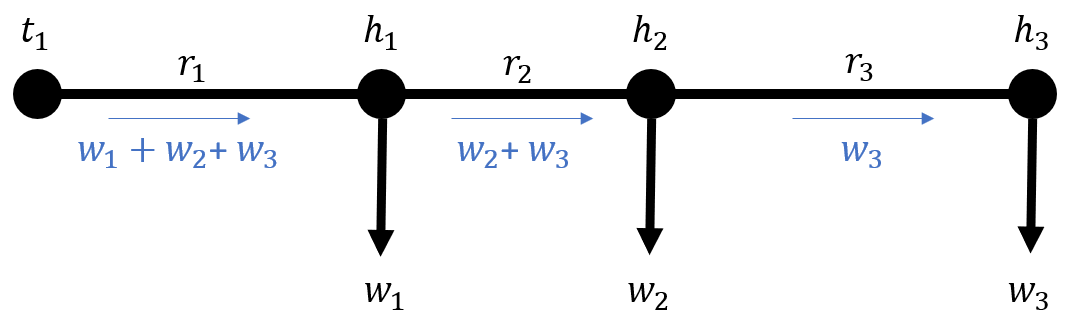
\includegraphics[width=\textwidth]{constraint-1}
	\caption{\color{blue}A \emph{house spider} with three houses and transformer at the root node. The voltage drop in each segment is proportional to the length of segment as well as the sum of loads at children nodes.}
	\label{fig-1}
\end{figure}
The voltage drop constraint is mathematically formulated in this section. Consider a leg of a \emph{house spider} as shown in Fig.~\ref{fig-1} with three houses $h_1,h_2,h_3$ and a transformer at the root $t_1$. The line segments connecting the nodes have a resistance of $r_1,r_2,r_3$ respectively and is proportional to the lengths. Each node barring the transformer has a weight given by $w_1,w_2,w_3$ which indicates the average load demand at the node. Assuming purely resistive network and power factor of unity (which is a reasonable assumption for planning purpose) the currents in each segment is proportional to the sum of weights in the leaf nodes. Therefore, the voltage drop along a segment is proportional to the product of its resistance and the current through it.

\begin{figure}[H]
	\centering
	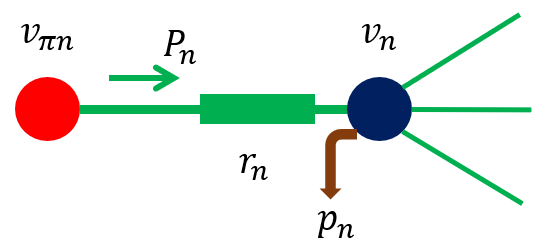
\includegraphics[width=0.5\textwidth]{constraint-2}
	\caption{\color{blue}Power balance constraints at a node $n$ along the \emph{house spider} with voltage $v_n$ and load $p_n$. The node has a parent node $\pi_n$.}
	\label{fig-2}
\end{figure}
\noindent We consider a node $n$ along the leg of the \emph{house spider} with a load of $p_n$ and voltage $v_n$. The node has a parent node with voltage $v_{\pi_n}$. Let the resistance of incident edge be given by $r_n$ and the power flowing through it be $P_n$. The edge to child node $k$ transmits power of $P_k$. The constraints are listed as follows.
\begin{equation}
\begin{aligned}
&v_{\pi_n}-v_n=i_nr_n\\
&P_n=v_{\pi_n}i_n\\
&P_n-i_n^2r_n-p_n=\sum_{k:n\rightarrow k}P_k
\end{aligned}
\end{equation}

\color{black}
\noindent
\textbf{Assumption:} A reasonable assumption is that possible cables that might connect the houses to transformers cannot exceed a certain length 
$CL$ due to engineering reasons. This places constraint on how these cables can be used. Another intuitive constraint appears to
be to try and preclude edges/cables that cross the road to connect houses as much as possible. So if houses $a,b,c$ are placed on one side of a street and $x,y,z$ on the other side in the same order then a path of the sort $a,x,b,y,c,z$ does not seem like a good path. On the other hand
$a,b,c,z$ might be okay as one house might be picked up in the path.  Let us call therefore have each edge comprise of two attributes:
a length $w_e$ and a label $l_e$.  The label has two possible \emph{crossing} and \emph{non-crossing}. We hope to find a solution that
does not have too many crossing edges (crossing the road) in each leg..

Please note that the constraints are as we understand the problem best; a lot of it is a matter of convention and best practices in the power industry. This means we need to verify this, second we should be ready to face a situation when this changes.

\noindent
\textbf{Formal problem:}  We are given a graph $G(V,E)$ 
comprising of a disjoint union of three class of nodes $H$, $T$, $S$, denoting Houses, transformers and substations respectively.
There is exactly one substation node $s$
The edges  $e \in E$ in the graph $G$ have an associated label $l_e$ and weight(length) $w_e$. We can assume that as a part of
constructing the feasible graph $G$, designers have kept exactly edges that are feasible, thus (i) there are no edges from  a house node
$h \in H$ to the substation $s$. Furthermore, only edges that are feasible (i.e. not too long) are part of the graph $G$.


Find a tree $T$ that is a subgraph of $G$ such that it has the following properties: (i) the length of the
spider legs is bounded by $L$, the total cost of all edges included in the tree is bounded by $B$, the total number of edges
in each of the spider leg, the total number of edges labeled as crossing edges is bounded by $C$ (usually 1 or 2).

\section{Complexity and a heuristic}

\noindent
\textbf{Complexity:}
This is a multi-criteria optimization problem and can be shown to be NP-hard in general I think by simple reduction from set cover.
(Add a super nodes, sets are possible transformers and edges are from transformers to houses. Covering the houses implies finding a good set cover and vice-versa). As a result is also hard to approximate.


\noindent
\textbf{A possible solution:}  One way to solve this problem is solve this where one finds a good spider cover to cover all houses and then
builds a core tree comprising of the root of the spiders and the substation. Ofcourse the choice of the substation used to connect the houses and then their connection to substation is coupled, and as a result the proposed solution below does not necessarily imply a provably good solution to the overall problem.

The spider cover can be simply thought of as a set cover problem: think of the spider root as a set and the elements it covers as all of them within a
distance of $L$ from it. One hopes that these nodes can be decomposed in a set of not heavily crossing chains. So you select the next spider head, cover the houses (choose the one that minimizes the total weight of the chains, not super clear for now) and then iterate.


\section{Proposed Methodology 1}
The first method considers the road network graph $\mathsf{R}=(\mathsf{V_R},\mathsf{E_R})$ and the set of home coordinates $\mathsf{H}$ together to generate the secondary distribution network. First the residential buildings are mapped to nodes of the road network. Let it be denoted by $g:\mathsf{H}\rightarrow\mathsf{V_R}$ and subsequently we can evaluate the inverse mapping $g^{-1}:\mathsf{V_R}\rightarrow\mathsf{H}$. We assign a label $\mathsf{L_H}(h)$ to each home $h\in\mathsf{H}$ to determine which side (first or second) of the nearest road link it is present.
\begin{equation}
\mathsf{L_H}(h)=
\begin{cases}
1,~~~ \textrm{if }h\textrm{ is on first side of road link}\\
-1,~ \textrm{if }h\textrm{ is on second side of road link}
\end{cases}
\end{equation}
It is assumed that the road nodes are the locations of transformers which are connected to the homes mapped to it. In order to construct the network, a fully connected graph $\mathsf{G}=(\mathsf{V},\mathsf{E})$ is considered where $\mathsf{V}=\{r\}\cup g^{-1}(r)$ for all $r\in\mathsf{V_R}$. If $g^{-1}(r)=\emptyset$, no secondary network is created for the road node. We assign a label $\mathsf{L}(v)$ to each node $v\in\mathsf{V}$ as
\begin{equation}
\mathsf{L}(v)=
\begin{cases}
\mathsf{L_H}(v),~\textrm{if }v\in\mathsf{H}\\
0,~~~~~~~ \textrm{if }v\in\mathsf{V_R}
\end{cases}
\end{equation}
The edges $(u,v)\in\mathsf{E}$ for all $u,v\in\mathsf{V}$ are assigned weights $w(u,v)$
\begin{equation}
w(u,v)=\mathsf{dist}(u,v)+\lambda \mathsf{C}(u,v)
\end{equation}
where $\mathsf{dist}:\mathsf{V}\times\mathsf{V}\rightarrow\mathbb{R}$ denotes the Euclidean distance between the residential locations $u,v$. The function $\mathsf{C}$ denotes if the edge crosses the nearest road link and is defined as
\begin{equation}
\mathsf{C}(u,v)=|\mathsf{L}(u)-\mathsf{L}(v)|=
\begin{cases}
0,\quad \textrm{if }u,v\textrm{ are on same side of road}\\
2,\quad \textrm{if }u,v\textrm{ are on opposite side of road}\\
1,\quad \textrm{if }u\in\mathsf{V_R}\textrm{ or }v\in\mathsf{V_R}
\end{cases}
\end{equation}
$\lambda$ is a weight factor to penalize multiple crossing of edges over the road links. It also penalizes multiple edges emerging from the root node. Thereafter, a minimum spanning tree (MST) rooted at the road nodes and spanning all the nodes of $\mathsf{G}$ is considered as the secondary network.
\begin{algorithm}
	\caption{Generating secondary distribution network based on road network}
	\label{alg:1}
	\begin{algorithmic}[1]
		\REQUIRE Mapping $g:\mathsf{H}\rightarrow\mathsf{V_R}$ between residential locations and road network nodes, labels $\mathsf{L}(h)$ for all homes $h\in\mathsf{H}$, penalty factor $\lambda$
		\STATE Compute the inverse mapping $g^{-1}:\mathsf{V_R}\rightarrow\mathsf{H}$ for all $r\in\mathsf{V_R}$ such that $g^{-1}(r)\neq\emptyset$.
		\FOR {$r\in\mathsf{V_R},~g^{-1}(r)\neq\emptyset$}
		\STATE Construct a fully connected graph $\mathsf{G}=(\mathsf{V},\mathsf{E})$ with $\mathsf{V}=\{r\}\cup g^{-1}(r)$ and edges $(u,v)$ with edge weights given by $w(u,v)$.
		\STATE Compute a MST $\mathsf{T_r}$ which spans all nodes in $\mathsf{G}$ and is rooted at $r$.
		\ENDFOR
		\STATE $\mathcal{F}=\{\mathsf{T_1},\mathsf{T_2},\cdots,\mathsf{T_r},\cdots,\}$ gives the secondary distribution network.
	\end{algorithmic}
\end{algorithm}
\begin{figure}[h]
	\centering
	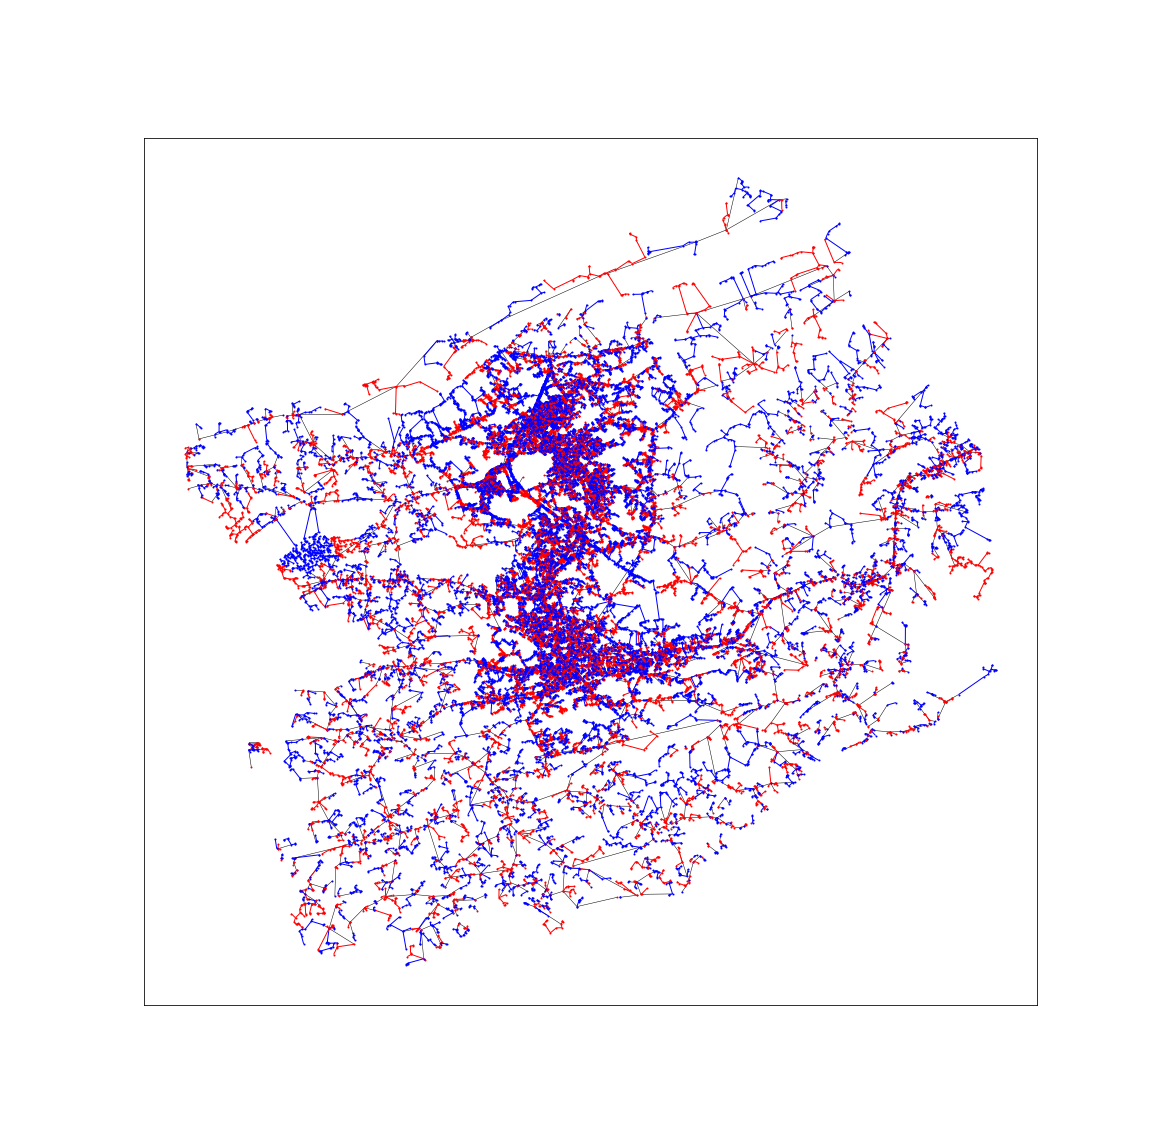
\includegraphics[width=\textwidth]{met-1}
	\caption{Secondary distribution network generated using the road network nodes as the location of transformers and considering a penalty factor of $\lambda=0.5$.}
	\label{fig:method-1}
\end{figure}

\begin{figure}[h]
	\centering
	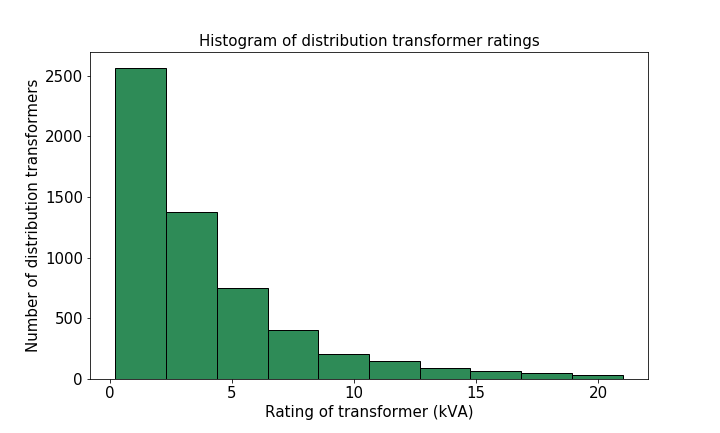
\includegraphics[width=\textwidth]{rating_dist}
	\caption{Histogram of distribution transformer ratings.}
	\label{fig:rating-method-1}
\end{figure}

\begin{figure}[h]
	\centering
	\begin{subfigure}[h]{0.32\textwidth}
		\centering
		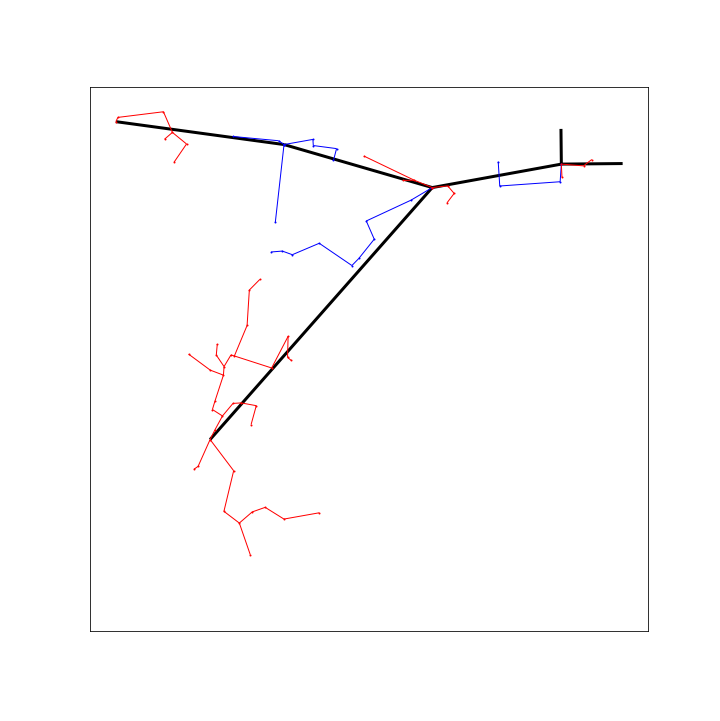
\includegraphics[width=\textwidth]{met-1-link1}
		\caption{}
		\label{sfig:link1}
	\end{subfigure}
	\begin{subfigure}[h]{0.32\textwidth}
		\centering
		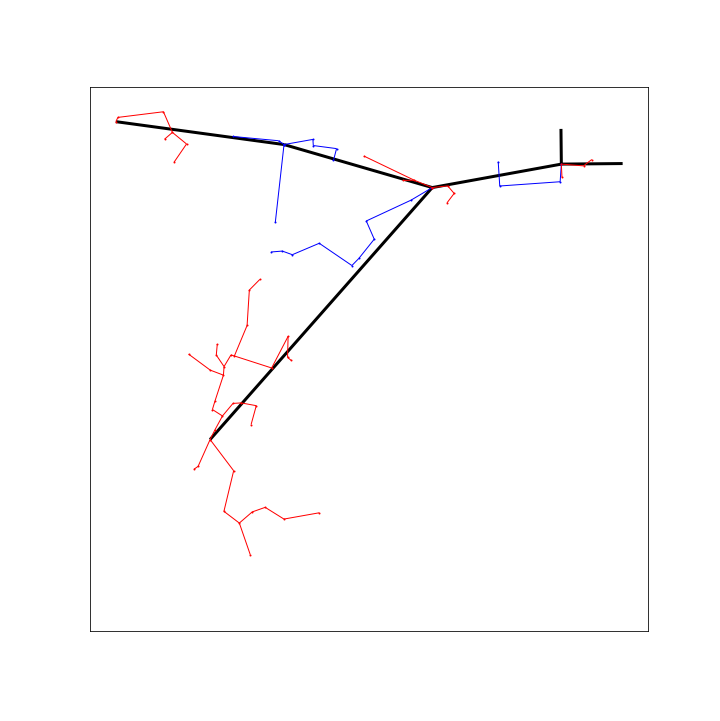
\includegraphics[width=\textwidth]{met-1-link1}
		\caption{}
		\label{sfig:link2}
	\end{subfigure}
	\begin{subfigure}[h]{0.32\textwidth}
		\centering
		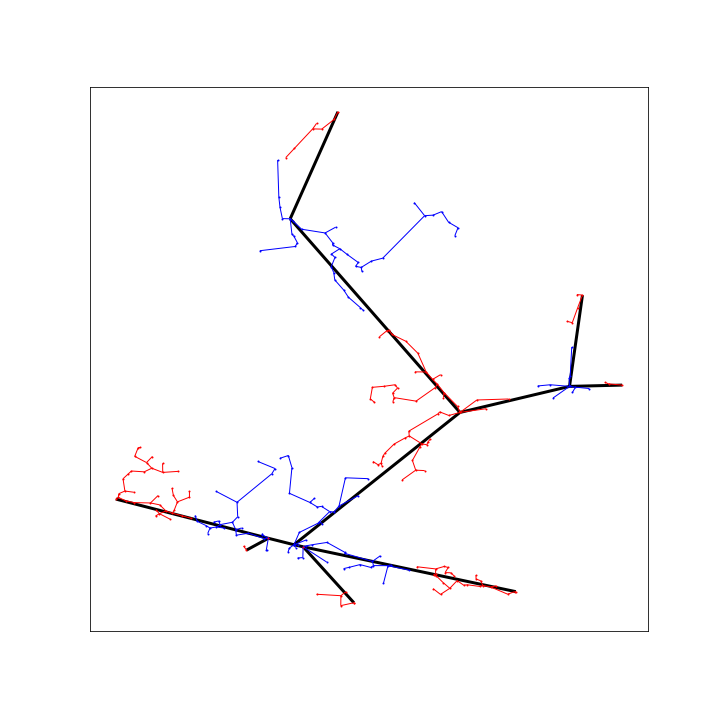
\includegraphics[width=\textwidth]{met-1-link3}
		\caption{}
		\label{sfig:link3}
	\end{subfigure}
	\caption{Secondary distribution generated using this method results in long branches from the root nodes. Furthermore, for long road links the branches become long as compared to surrounding smaller links.}
	\label{fig:method1links}
\end{figure}

\newpage
\section{Proposed Methodology 2}
This method constructs the secondary distribution network without any information about the road network. However, it takes into account the power system constraints like maximum allowable rating of distribution transformers and number of customers served by each transformer. For this method, we require the load demand profile for each residential building. We can compute the average hourly load demand for each residential building using $\underline{D_{h}}=\sum_{i=1}^{24}d_{h,i}$ where $d_{h,i}$ is the hourly load demand at home $h$ for the $i^{th}$ hour. This average load is considered as the weight for the corresponding home. We perform a weighted k-means clustering over the spatial locations of the residential buildings such that for each iteration the centroid of cluster $c$ with $N_c$ home points is updated as
\begin{equation}
\underline{x_c}=\dfrac{1}{N_c}\sum_{h=1}^{N_c}x_h\underline{D_{h}}\quad \textrm{and} \quad\underline{y_c}=\dfrac{1}{N_c}\sum_{h=1}^{N_c}y_h\underline{D_{h}}
\end{equation}
We undertake an iterative procedure with minimum number of clusters given by
\begin{equation}
k_{min}=\dfrac{\textrm{Total load to be served}}{\textrm{maximum allowable rating}}=\dfrac{\sum_{h\in\mathsf{H}}{\underline{D_h}}}{\mathsf{P_{max}}}
\end{equation}
After weighted k-means clustering is performed, the constraints are checked, that is if the transformer ratings do not exceed a specified limit or number of customers served by a transformer exceeds a threshold. If any constraint is violated, the number of clusters are increased and the weighted k-means algorithm is applied again.

\begin{algorithm}
	\caption{Generating secondary distribution network using weighted k-means clustering}
	\label{alg:2}
	\begin{algorithmic}[1]
		\REQUIRE Load demand profile $\{d_{h,i}\}_{i=1}^{24}$ for all $h\in\mathsf{H}$, maximum allowable transformer rating $\mathsf{P_{max}}$.
		\STATE Compute the minimum number of transformers required $k_{min}$ and assign $k\leftarrow k_{min}$.
		\STATE Assign to each home $h\in\mathsf{H}$ its average hourly load demand $\underline{D_h}$ as corresponding weight.
		\STATE Perform weighted k-means clustering on all homes $h\in\mathsf{H}$ with $k$ clusters.
		\STATE Compute the ratings of $k$ transformers.
		\IF {maximum rating exceeds $\mathsf{P_{max}}$}
		\STATE Increment $k$ and go to Step 3.
		\ENDIF
		\STATE Finalize the $k$ clusters and assign transformers to centroids of the $k$ clusters.
		\STATE Compute a MST $\mathsf{T_i}, i=1,2,\cdots,k$ for each of the $k$ clusters which spans the homes in the cluster and is rooted at the centroid.
		\STATE The centroids are connected to the nearest point on the road network to complete the connection between secondary and primary networks.
		\STATE $\mathcal{F}=\{\mathsf{T_1},\mathsf{T_2},\cdots,\mathsf{T_r},\cdots,\}$ gives the secondary distribution network.
	\end{algorithmic}
\end{algorithm}
\end{document}